\chapter{Spécificités du Réseau Routier Béninois et Rôle des Motos}
\label{chap:specificites_benin}

\section{Diversité des Infrastructures au Bénin}
\label{sec:diversite_infrastructures}

Le réseau routier béninois présente une grande hétérogénéité qui impacte significativement la dynamique du trafic. Cette diversité se manifeste à plusieurs niveaux : qualité du revêtement, largeur des voies, présence ou absence de trottoirs, et organisation des intersections.

\subsection{Types de Revêtement et État des Routes}
\label{subsec:types_revetement}

Selon les données de la Banque Mondiale \cite{worldbank2019benin}, le réseau routier béninois totalise environ 18 500 km, dont seulement 9,7\% (1 800 km) sont pavés à l'échelle nationale. Cette proportion varie significativement entre les zones rurales et urbaines. Le réseau comprend quatre principales catégories de revêtement, chacune influençant différemment la circulation des véhicules :

\begin{itemize}
\item \textbf{Routes bitumées} : Principalement présentes dans les grandes villes et sur les axes interurbains majeurs, elles peuvent représenter jusqu'à 30-35\% du réseau urbain dans des villes comme Cotonou. Leur qualité varie considérablement, allant de voies rapides bien entretenues à des routes fortement dégradées avec nids-de-poule.

\item \textbf{Routes en terre} : Constituant la majorité du réseau national, ces routes non revêtues sont particulièrement sensibles aux conditions climatiques. En saison sèche, elles génèrent de la poussière affectant la visibilité, tandis qu'en saison des pluies, elles deviennent souvent boueuses et difficilement praticables pour les voitures, mais restent accessibles aux motos.

\item \textbf{Routes pavées} : Présentes dans certaines zones urbaines et périurbaines, ces routes offrent une bonne adhérence mais créent des vibrations qui ralentissent les véhicules, particulièrement les voitures, alors que les motos y maintiennent une vitesse plus élevée.

\item \textbf{Pistes et voies informelles} : Ces chemins, souvent créés par l'usage répété, sont généralement inaccessibles aux voitures mais fréquemment empruntés par les motos, créant un réseau parallèle non officiel.
\end{itemize}

\begin{figure}[htbp]
\centering
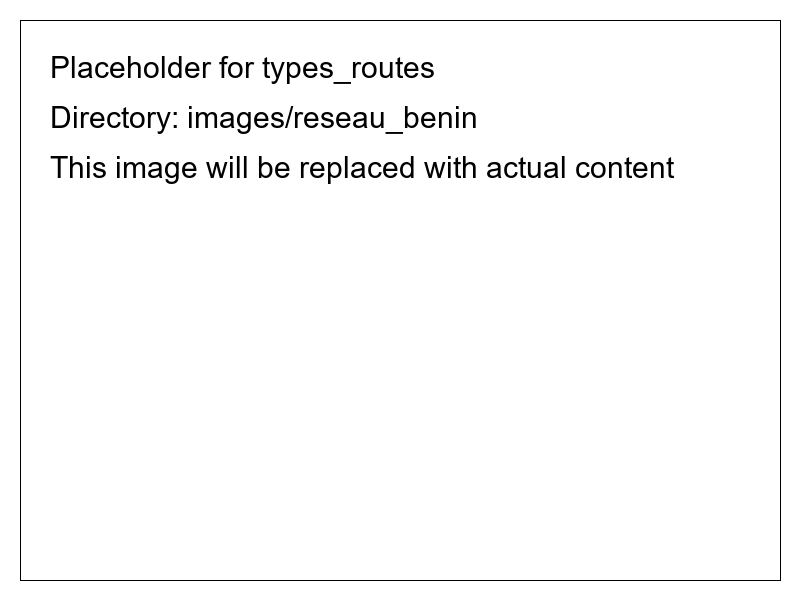
\includegraphics[width=0.9\textwidth]{images/reseau_benin/types_routes}
\caption{Les différents types de routes au Bénin : (a) route bitumée à Cotonou; (b) route en terre en zone périurbaine; (c) route pavée; (d) piste accessible uniquement aux motos.}
\label{fig:types_routes}
\end{figure}

\begin{remark}
Cette diversité des revêtements routiers affecte différemment chaque classe de véhicule, les motos étant généralement moins impactées par la dégradation du revêtement que les voitures, ce qui nécessitera une prise en compte spécifique dans notre modélisation.
\end{remark}

\subsection{Organisation Spatiale du Réseau}
\label{subsec:organisation_spatiale}

La configuration du réseau routier béninois présente plusieurs particularités structurelles :

\begin{itemize}
\item \textbf{Structure radiale} dans les grandes villes comme Cotonou, avec des axes principaux convergeant vers le centre, créant des points de congestion.

\item \textbf{Voies à largeur variable} : La largeur des routes change fréquemment, créant des goulots d'étranglement où s'accumulent les véhicules. Ces variations affectent différemment les classes de véhicules, les motos étant moins impactées.

\item \textbf{Rareté des voies rapides dédiées} : Le réseau compte peu d'autoroutes ou voies rapides dédiées, ce qui limite la séparation des flux de véhicules selon leur vitesse.

\item \textbf{Zones d'habitat spontané} créant des réseaux irréguliers où coexistent véhicules et piétons, avec une forte présence de motos.
\end{itemize}

\subsection{Gestion des Intersections}
\label{subsec:gestion_intersections}

Les intersections au Bénin présentent des spécificités qui complexifient leur modélisation :

\begin{itemize}
\item \textbf{Faible présence de feux de circulation} : Moins de 20\% des intersections urbaines sont régulées par des feux, souvent sujets à des pannes. Cette situation est caractéristique de nombreuses villes d'Afrique subsaharienne \cite{loggoh2019traffic}.

\item \textbf{Ronds-points surchargés} : Les ronds-points, nombreux dans les villes, deviennent des points de congestion majeurs aux heures de pointe.

\item \textbf{Prédominance de la priorité à droite} ou de la négociation informelle entre conducteurs.

\item \textbf{Présence d'agents de circulation} aux intersections majeures, introduisant une variabilité humaine dans la régulation.
\end{itemize}

\begin{figure}[htbp]
\centering
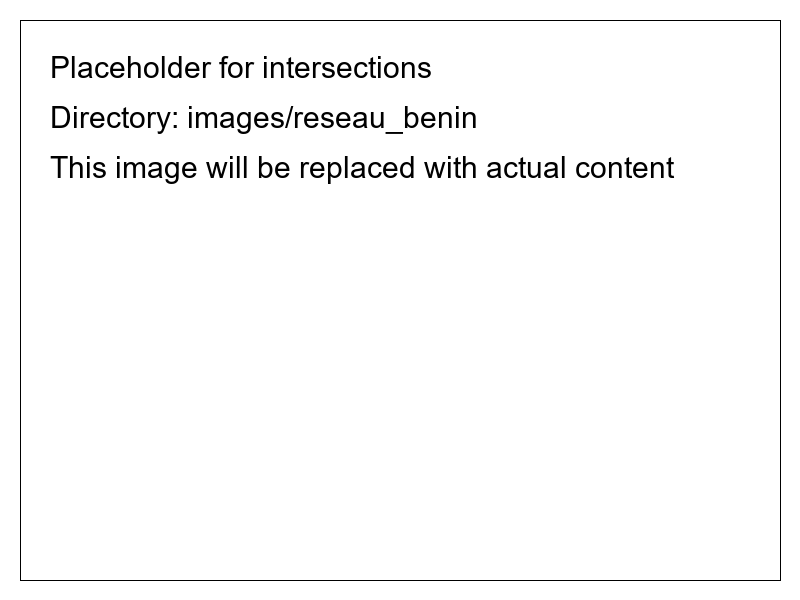
\includegraphics[width=0.8\textwidth]{images/reseau_benin/intersections}
\caption{Gestion des intersections au Bénin : (a) carrefour sans feux avec agent de circulation; (b) rond-point congestionné; (c) intersection non régulée avec motos prédominantes.}
\label{fig:intersections}
\end{figure}

\begin{theorem}[Modélisation des intersections béninoises]
Dans notre modèle, une intersection sera représentée par un terme source/puits $S_i(x,t)$ dans l'équation de conservation, avec :
\begin{align}
S_i(x,t) = \alpha_i(t) \cdot \delta(x-x_0)
\end{align}
où $\alpha_i(t)$ représente le flux entrant/sortant de véhicules de classe $i$, $\delta$ est la distribution de Dirac, et $x_0$ la position de l'intersection.
\end{theorem}

\section{Collecte et Exploitation des Données Béninoises}
\label{sec:collecte_donnees}

La modélisation précise du trafic béninois nécessite des données spécifiques au contexte local.

\subsection{Méthodologie de Collecte des Données}
\label{subsec:methodologie_collecte}

En raison de limitations pratiques et logistiques, notre approche de collecte de données s'appuie principalement sur les sources suivantes :

\begin{itemize}
\item \textbf{Données de Google Maps Traffic Layer} : Cette source constitue notre outil principal, fournissant des informations en temps réel sur la congestion et les vitesses moyennes sur différents axes routiers. L'API de Google Maps permet d'extraire des données historiques de trafic à différentes heures de la journée et jours de la semaine, offrant une vision dynamique des conditions de circulation. Nous utilisons ces données pour :
  \begin{itemize}
    \item Identifier les zones de congestion récurrentes
    \item Estimer les vitesses moyennes sur différents types de routes
    \item Observer les variations temporelles (heures de pointe, différences jour/nuit, jours ouvrables/week-end)
    \item Évaluer l'impact des conditions météorologiques sur le trafic
  \end{itemize}

\item \textbf{Données statistiques officielles} du Ministère des Transports du Bénin et de l'Institut National de la Statistique et de l'Analyse Économique (INSAE), notamment pour la composition du parc automobile et la répartition des types de véhicules.

\item \textbf{Littérature existante et études antérieures}, particulièrement les travaux de \cite{loggoh2019traffic} et \cite{aerc2019taxi}, qui fournissent des informations précieuses sur les comportements de conduite et les spécificités du trafic béninois.

\item \textbf{Observations qualitatives} documentées sous forme de photographies et notes descriptives lors de visites sur le terrain, sans mesures quantitatives systématiques.

\item \textbf{Consultation d'experts locaux} et de professionnels du transport, notamment des urbanistes, des ingénieurs en transport et des responsables de la sécurité routière, qui ont partagé leurs connaissances et expériences.
\end{itemize}

\begin{remark}
Bien que cette approche présente des limitations, notamment l'absence de données détaillées sur la composition exacte du trafic et les comportements spécifiques des différentes classes de véhicules, elle permet néanmoins d'obtenir une vision globale des dynamiques de circulation au Bénin.
\end{remark}

\subsection{Traitement et Analyse des Données}
\label{subsec:traitement_donnees}

Malgré les limitations dans la collecte, nous avons développé une méthodologie adaptée pour exploiter au mieux les données disponibles :

\begin{enumerate}
\item \textbf{Extraction systématique des données de Google Maps} à intervalles réguliers (toutes les heures pendant plusieurs semaines) pour constituer une base temporelle représentative.

\item \textbf{Classification des segments routiers} selon leur type (bitumé, terre, pavé) basée sur les données cartographiques et les observations qualitatives.

\item \textbf{Analyse des variations temporelles} pour identifier les motifs récurrents de congestion et estimer les densités relatives de trafic.

\item \textbf{Croisement avec les données statistiques officielles} pour inférer la composition probable du trafic dans différentes zones et à différentes périodes.

\item \textbf{Validation par triangulation} avec les observations qualitatives et les informations issues de la littérature existante.
\end{enumerate}

\section{Spécificités des Types de Véhicules et Place des Motos}
\label{sec:specificites_vehicules}

\subsection{Hétérogénéité du Parc Automobile}
\label{subsec:heterogeneite_parc}

Le parc automobile béninois présente une grande diversité qui impacte la dynamique du trafic. Selon les études disponibles, notamment celle de l'AERC \cite{aerc2019taxi}, la composition du trafic se caractérise par :

\begin{itemize}
\item \textbf{Motos et motocyclettes} (localement appelées "Zémidjans" lorsqu'elles servent de taxi) : Représentant plus de 70\% des véhicules en circulation, elles constituent l'épine dorsale du transport urbain \cite{aerc2019taxi}.

\item \textbf{Voitures particulières} : Environ 15\% du parc, composé de véhicules d'âges et de tailles variés, souvent importés d'occasion.

\item \textbf{Taxis-ville} (généralement des berlines peintes en jaune) : Environ 5\% du parc dans les zones urbaines.

\item \textbf{Minibus et bus} : Services de transport en commun, représentant 3\% des véhicules.

\item \textbf{Camions et poids lourds} : Environ 7\% des véhicules, principalement sur les axes interurbains et les zones portuaires.
\end{itemize}

Cette hétérogénéité se traduit par des différences significatives dans les paramètres de conduite, comme illustré dans le tableau suivant :

\begin{table}[htbp]
\centering
\caption{Paramètres caractéristiques par classe de véhicule}
\label{tab:parametres_vehicules}
\begin{tabular}{lcccc}
\toprule
\textbf{Classe} & \textbf{$v_{i,\max}^0$ (km/h)} & \textbf{$\rho_{i,\max}$ (véh/km)} & \textbf{Coefficient $\mu_i$} & \textbf{Impact relatif} \\
 & & & & \textbf{du type de route} \\
\midrule
Motos & 60 & 240 & -- & 1.0 \\
Voitures & 70 & 180 & 0.3 & 0.7 \\
Taxis & 65 & 180 & 0.4 & 0.8 \\
Bus & 55 & 140 & 0.5 & 0.6 \\
Camions & 50 & 120 & 0.6 & 0.5 \\
\bottomrule
\end{tabular}
\end{table}

\subsection{Rôle Prépondérant des Motos dans le Trafic Béninois}
\label{subsec:role_motos}

Les motos jouent un rôle central dans le trafic béninois qui les distingue fondamentalement des autres classes de véhicules. Les études comme celles de \cite{loggoh2019traffic} et \cite{aerc2019taxi} confirment leur prédominance et leurs comportements spécifiques :

\begin{itemize}
\item \textbf{Capacité d'infiltration} : Les motos peuvent s'insérer dans des espaces réduits entre les voitures, créant un flux qui s'écoule même en situation apparemment congestionnée \cite{kumar2018motorcycle}.

\item \textbf{Trajectoires flexibles} : Contrairement aux voitures confinées à leurs voies, les motos suivent des trajectoires opportunistes, changeant fréquemment de direction.

\item \textbf{Comportement collectif} : Les motos tendent à se regrouper aux feux rouges et intersections, formant des "essaims" qui démarrent rapidement au feu vert.

\item \textbf{Adaptation aux infrastructures dégradées} : Les motos peuvent maintenir une vitesse relativement élevée sur des surfaces où les voitures doivent considérablement ralentir \cite{karthik2019estimation}.
\end{itemize}

\begin{definition}[Gap-filling]
Le comportement gap-filling désigne la capacité des motos à occuper les espaces entre les véhicules plus grands, augmentant ainsi la densité effective du trafic sans nécessairement réduire les vitesses \cite{fan2013heterogeneous}.
\end{definition}

\begin{definition}[Interweaving]
Le comportement interweaving désigne le mouvement en zigzag des motos entre les files de véhicules, créant un flux transversal qui peut perturber l'écoulement des autres classes \cite{kumar2018motorcycle}.
\end{definition}

Ces comportements spécifiques nécessitent une modélisation dédiée dans notre extension du modèle LWR, notamment à travers des fonctions de modulation qui seront introduites dans le chapitre suivant.

\begin{figure}[htbp]
\centering
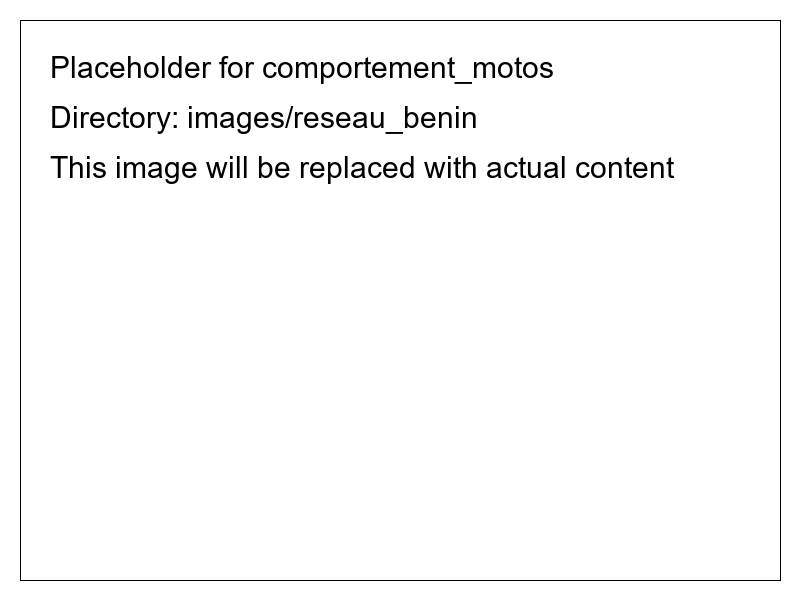
\includegraphics[width=0.9\textwidth]{images/reseau_benin/comportement_motos}
\caption{Comportements spécifiques des motos dans le trafic béninois : (a) gap-filling entre voitures; (b) regroupement aux intersections; (c) trajectoires flexibles contournant les obstacles.}
\label{fig:comportement_motos}
\end{figure}

\subsection{Impact des Motos sur la Dynamique Globale du Trafic}
\label{subsec:impact_motos}

La prédominance des motos modifie profondément la dynamique du trafic par rapport aux modèles classiques. Les études de \cite{wong2002multi} et \cite{fan2013heterogeneous} ont démontré plusieurs impacts significatifs :

\begin{itemize}
\item \textbf{Augmentation de la capacité effective} des routes : En utilisant l'espace disponible de manière plus efficace, les motos permettent d'accroître le flux total de véhicules \cite{chanut2005modeles}.

\item \textbf{Modification des relations vitesse-densité} : La présence de nombreuses motos peut maintenir des vitesses moyennes relativement élevées même à forte densité totale, contrairement au modèle classique de Greenshields \cite{greenshields1935study}.

\item \textbf{Transformation des intersections} en points de mélange complexe où les principes habituels de priorité sont souvent remplacés par une négociation constante entre usagers \cite{akcelik2003relationship}.

\item \textbf{Création de réseaux parallèles informels} : Les motos empruntent souvent des chemins inaccessibles aux autres véhicules, redistribuant le trafic de manière difficile à prédire avec les modèles classiques.
\end{itemize}

\begin{proposition}
Dans un flux mixte avec une proportion significative de motos, la relation entre la densité totale $\rho$ et le flux total $q$ n'est plus une fonction simple comme dans le modèle de Greenshields \cite{greenshields1935study}, mais dépend de la composition du trafic :
\begin{align}
q(\rho, \rho_M) = \sum_{i=1}^N \rho_i \cdot v_i(\rho, \rho_M)
\end{align}
où $\rho_M$ est la densité des motos, et les fonctions $v_i$ intègrent l'effet des motos sur chaque classe.
\end{proposition}

\section{Vers un Modèle Adapté aux Spécificités Béninoises}
\label{sec:vers_modele_adapte}

Les spécificités du réseau routier béninois et le rôle particulier des motos nécessitent une adaptation profonde des modèles de trafic standards comme le modèle LWR \cite{lighthill1955kinematic, richards1956shock}.

\begin{itemize}
\item La \textbf{diversité des infrastructures} exige l'introduction de facteurs spécifiques à chaque type de route et classe de véhicule dans notre modèle.

\item L'\textbf{hétérogénéité du parc automobile} justifie une approche multiclasses avec des paramètres distincts pour chaque type de véhicule, comme proposé par \cite{wong2002multi}.

\item Le \textbf{comportement spécifique des motos} requiert des fonctions de modulation traduisant leur impact sur les autres classes de véhicules, s'inspirant des approches de \cite{zhang2003non}.

\item La \textbf{gestion particulière des intersections} nécessite un traitement mathématique adapté des conditions aux limites et des termes sources/puits, comme suggéré par \cite{daganzo1995cell}.
\end{itemize}

Dans le chapitre suivant, nous développerons un cadre mathématique intégrant ces spécificités dans une extension du modèle LWR qui représentera fidèlement la dynamique du trafic routier au Bénin.
